\section{Resultados}
\label{sec:ModelosFuncionales}

\subsection{Pruebas de usuario}

Se han realizado \textbf{pruebas de usuario} para comprobar si los resultados obtenidos se perciben como naturales. La obtención de feedback por parte de usuarios de videojuegos podría confirmar qué aspectos de la tela se han conseguido replicar y dónde se deberían producir mejoras.
ANEXO CUESTIONARIO

BLABLABLA

\subsection{Resultados visuales de la inferencia}
En este apartado se muestran ejemplos comparando la tela simulada por Unity y la inferencia que el modelo consigue. \newline
\subsubsection{Entrenamiento movimiento lineal}
En el caso de los modelos entrenados con un movimiento lineal, la inferencia es casi perfecta con un entrenamiento muy sencillo.

\subsubsection{Entrenamiento movimiento aleatorio}
En el caso de los modelos entrenados con aleatoriedad en el movimiento del colisionador, que se describen en el apartado \ref{subsec:sim}, puede conseguirse un resultado adecuado pero requiere de un entrenamiento mucho más costoso. 

Este movimiento se probó entrenando dos modelos con los mismos parámetros: uno con los parámetros de posición y SDF, y otro con la velocidad añadida. Se descartó el modelo entrenado con velocidad, que pese ser el modelo que obtiene mejores resultados en este entrenamiento, con un error medio por vértice de 0.000923m, en Unity no logra mantener la estructura de la tela. Pese a que la tela consigue replicar el movimiento pendular adecuado, y no se rompe por completo durante toda la duración de la simulación, se forman en la tela picos o deformaciones incorrectas que rompen la coherencia visual por completo. %insertese foto%.

Hiiii 

\begin{table}[H]
    \begin{center}
        \begin{tabular}{ | m{2.2cm} | m{2cm} | m{1.2cm} | m{2.1cm} | m{2.4cm} | m{2.2cm} | }
        \hline \textbf{Windows size} & \textbf{Rollout steps} & \textbf{Noise} & \textbf{Learning rate} & \textbf{Tamaño dataset} & \textbf{Batch size} \\ \hline
            16 & 24 & 3\% & 0.001 & 25000 & 32 \\ \hline
        \end{tabular}
            \end{center}
    \caption{Hiperparámetros y configuración del entrenamiento Vel.}
    \label{tab:randomTraining}
\end{table}
        
\begin{table}[H]
    \begin{center}
        \begin{tabular}{ | m{3cm} | m{3cm} | m{1.2cm} | m{2cm} | }
        \hline \textbf{Tiempo} & \textbf{Error medio por vertice} & \textbf{FPS} & \textbf{Percepción} \\ \hline
            20h(gpu) & 0.000923 & 110 & 8/10 \\ \hline
        \end{tabular}
    \end{center}
    \caption{Resultados del entrenamiento Vel.}
    \label{tab:randomResults}
\end{table}

Por ende, se realizan finalmente las pruebas de entrenamiento y visualización finales sobre el modelo que recibe como parámetros de entrada la posición de los vértices y el SDF. Se llevan a cabo tres iteraciones de la prueba, con objeto de encontrar el balance entre tasa de frames alcanzada y calidad de la recreación de la tela. Estas tres pruebas se realizan manteniendo los mismos parámetros descritos en la tabla  x, e incrementando sobre la secuencia de longitud que toma el modelo en la recurrencia. 

En las siguientes tablas y figuras, \ref{tab:randomTraining}, \ref{fig:inferenciaRandom} y \ref{fig:realRandom}, se muestran estos resultados. Puede apreciarse que la bola atraviesa la tela en ocasiones, esto se debe a las limitaciones del entrenamiento pero también a las de la propia simulación de Cloth, ya que el solver de Unity comete errores de solapamiento igualmente.

\begin{table}[H]
    \begin{center}
        \begin{tabular}{ | m{2.2cm} | m{2cm} | m{1.2cm} | m{2.1cm} | m{2.4cm} | m{2.2cm} | }
        \hline \textbf{Windows size} & \textbf{Rollout steps} & \textbf{Noise} & \textbf{Learning rate} & \textbf{Tamaño dataset} & \textbf{Batch size} \\ \hline
            16 & 24 & 3\% & 0.001 & 25000 & 32 \\ \hline
        \end{tabular}
         \end{center}
    \caption{Hiperparámetros y configuración del entrenamiento.}
    \label{tab:randomTrainHip}
\end{table}

\begin{table}[H]
    \begin{center}
        \begin{tabular}{ | m{3cm} | m{3cm} | m{1.2cm} | }
        \hline \textbf{Tiempo} & \textbf{Error medio por vertice} & \textbf{FPS} \\ \hline
            18h & 0.0019 & 110 \\ \hline
        \end{tabular}
    \end{center}
    \caption{Resultados del entrenamiento.}
    \label{tab:randomTrainRes}
\end{table}

\begin{figure}[H]
    \centering
    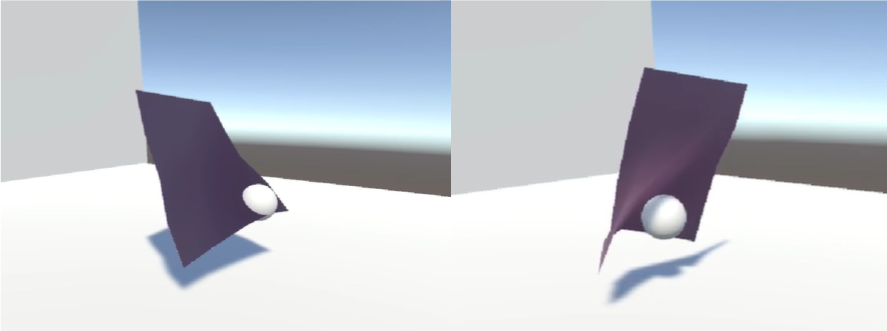
\includegraphics[width=0.9\textwidth]{Imagenes/inferenciaRandom.png}
    \caption{Inferencia del modelo para una muestra aleatoria.}
    \label{fig:inferenciaRandom}
\end{figure}
\begin{figure}[H]
    \centering
    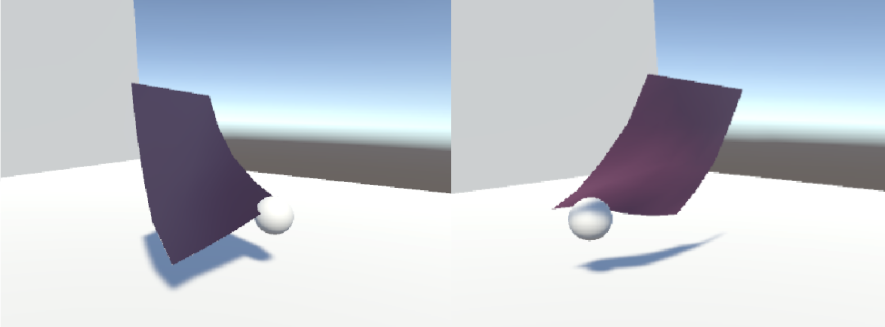
\includegraphics[width=0.9\textwidth]{Imagenes/realRandom.png}
    \caption{Simulación de Unity para una muestra aleatoria.}
    \label{fig:realRandom}
\end{figure}